
%% bare_conf.tex
%% V1.3
%% 2007/01/11
%% by Michael Shell
%% See:
%% http://www.michaelshell.org/
%% for current contact information.
%%
%% This is a skeleton file demonstrating the use of IEEEtran.cls
%% (requires IEEEtran.cls version 1.7 or later) with an IEEE conference paper.
%%
%% Support sites:
%% http://www.michaelshell.org/tex/ieeetran/
%% http://www.ctan.org/tex-archive/macros/latex/contrib/IEEEtran/
%% and
%% http://www.ieee.org/

%%*************************************************************************
%% Legal Notice:
%% This code is offered as-is without any warranty either expressed or
%% implied; without even the implied warranty of MERCHANTABILITY or
%% FITNESS FOR A PARTICULAR PURPOSE!
%% User assumes all risk.
%% In no event shall IEEE or any contributor to this code be liable for
%% any damages or losses, including, but not limited to, incidental,
%% consequential, or any other damages, resulting from the use or misuse
%% of any information contained here.
%%
%% All comments are the opinions of their respective authors and are not
%% necessarily endorsed by the IEEE.
%%
%% This work is distributed under the LaTeX Project Public License (LPPL)
%% ( http://www.latex-project.org/ ) version 1.3, and may be freely used,
%% distributed and modified. A copy of the LPPL, version 1.3, is included
%% in the base LaTeX documentation of all distributions of LaTeX released
%% 2003/12/01 or later.
%% Retain all contribution notices and credits.
%% ** Modified files should be clearly indicated as such, including  **
%% ** renaming them and changing author support contact information. **
%%
%% File list of work: IEEEtran.cls, IEEEtran_HOWTO.pdf, bare_adv.tex,
%%                    bare_conf.tex, bare_jrnl.tex, bare_jrnl_compsoc.tex
%%*************************************************************************

\documentclass[conference]{IEEEtran}


% \usepackage[caption=false]{caption}
% \usepackage[font=footnotesize]{subfig}
% subfig.sty, also written by Steven Douglas Cochran, is the modern
% replacement for subfigure.sty. However, subfig.sty requires and
% automatically loads Axel Sommerfeldt's caption.sty which will override
% IEEEtran.cls handling of captions and this will result in nonIEEE style
% figure/table captions. To prevent this problem, be sure and preload
% caption.sty with its "caption=false" package option. This is will preserve
% IEEEtran.cls handing of captions. Version 1.3 (2005/06/28) and later
% (recommended due to many improvements over 1.2) of subfig.sty supports
% the caption=false option directly:
\usepackage[caption=false,font=footnotesize]{subfig}


% *** PDF, URL AND HYPERLINK PACKAGES ***
\usepackage{url}
% url.sty was written by Donald Arseneau. It provides better support for
% handling and breaking URLs. url.sty is already installed on most LaTeX
% systems. The latest version can be obtained at:
% http://www.ctan.org/tex-archive/macros/latex/contrib/misc/
% Read the url.sty source comments for usage information. Basically,
% \url{my_url_here}.

\usepackage{graphicx}
\usepackage{hyperref}
\usepackage{footnote}
\usepackage{listings}
\usepackage{dirtree}

\begin{document}
%
% paper title
% can use linebreaks \\ within to get better formatting as desired
\title{File Propagation Through Amazon CloudFront}


% author names and affiliations
% use a multiple column layout for up to three different
% affiliations
\author{\IEEEauthorblockN{Timo Saarinen}
\IEEEauthorblockA{School of Science\\
Aalto University\\
Email: timo.l.saarinen@aalto.fi}
\and
\IEEEauthorblockN{Martijn Roo}
\IEEEauthorblockA{School of Science\\
Aalto University\\
Email: martijn.roo@aalto.fi}}


% make the title area
\maketitle

\IEEEpeerreviewmaketitle



\section{Introduction}
Amazon CloudFront is service that provides a content delivery network (CDN). A CDN is a geographically wide network of computer nodes that makes it possible to distribute content to end users with low latency and high data transfer speeds. As of November 2014, Amazon CloudFront has edge locations in all continents except Africa and Antarctica. Most of them reside in USA, Europe and Asia \cite{CloudFront_product_details}.

This research aims to achieve a better understanding of how files propagate within Amazon CloudFront after a CloudFront distribution is created.  Multiple files of different sizes are made available through Amazon CloudFront and for these files the network latency and retrieval latency were measured from different, geographically spread-out locations at multiple times after initiating the CloudFront distribution. Here, the retrieval latency is the time from the first HTTP GET request until the first response packet that contains data.

\section{Experiment setup}
To setup the required cloud services, Amazon S3 buckets were created for each available location: US East, US West (Oregon), US West (California), Ireland, Frankfurt, Singapore, Sydney, Tokyo, and Sao Paulo. The S3 buckets functioned as storages for the files to be downloaded via CloudFront. Then, for each of those buckets, we created a CloudFront download distribution. Thus, all CDN download distributions had their own S3 origin in the same region. All download distributions were set to use only HTTP and to be available at all edge locations. Finally, five different-sized files were uploaded to each S3 bucket. The sizes were 1KB, 10KB, 100KB, 1MB, and 10MB. These files were made using rdfc, a Windows utility to make random binary data files of specific sizes.

\section{Measurements}
To capture how files of different sizes propagate through Amazon's CloudFront CDN network, we measured the network latency to the different CloudFront servers as well as the retrieval latency for each of the files at intervals of one hour starting after initializing the CloudFront distributions and continuing for approximately twenty measurements. These measurements were made from a home computer (located in Helsinki, Finland) and from Amazon EC2 instances in California, Ireland and Singapore.


Since we had 9 different S3 locations, 5 different file sizes, about 20 different measurement times, and 4 different measuring locations, there were numerous combinations. We used a CRON job to execute a bash script every hour at each of the four measurement locations. This bash script pings all the CloudFront distributions and retrieves the different files from all distributions while making a tshark log. Aggregating all the measurements resulted in the following file structure:\\

\dirtree{%
.1 d2dx94olpiqj0t.CloudFront.net.
.2 california.
.3 1kb.
.4 1kb\_19.11-17.40.txt.
.4 1kb\_19.11-18.40.txt.
.4 ....
.3 10kb.
.3 100kb.
.3 1mb.
.3 10mb.
.3 1kb.
.3 ping\_19.11-17.40.txt.
.3 ping\_19.11-18.40.txt.
.3 ....
.2 home.
.3 ....
.2 ireland.
.3 ....
.2 singapore.
.3 ....
.1 d3kjdkfj34jfd.CloudFront.net.
.2 ....
.1 ....
}

Another bash script extracts information from the raw logs created during measurements. This resulted in a CSV file containing columns shown in Table \ref{table:extracteddata}. The IP addresses are taken from the first HTTP response packet in the tshark logs of the 10mb file download. The network latencies are averages of pinging. Retrieval latencies are the durations between the first HTTP GET request and the first HTTP response packet in the tshark logs.

\begin{table*}
\renewcommand{\arraystretch}{1.3}
\caption{Extracted data}
\centering
\begin{tabular}{|c|c|c|c|c|c|c|c|c|c|c|}
\hline
\bfseries Measuring location & \bfseries id & \bfseries Datetime & \bfseries S3 location & \bfseries IP address & \bfseries Network latency & \bfseries 1KB (retr. latency) & \bfseries 10kb & \bfseries 100kb & \bfseries 1mb & \bfseries 10mb \\
\hline\hline
home & 0 & 16.11-14.00 & oregon & 54.230.99.246 & 34 & .031158 & .028388 & .028209 & .026788 & .037260 \\
\hline
home & 1 & 16.11-15.00 & oregon & 54.230.98.223 & 41 & .035771 & .035264 & .029972 & .035058 & .027095 \\
\hline
... & ... & ... & ... & ... & ... & ... & ... & ... & ... & ... \\
\hline
\end{tabular}
\label{table:extracteddata}
\end{table*}

\section{Results}
Relative changes in network latencies are visualized in \autoref{fig:ping_relative}. For every measurement location, three download distribution from different continents were used: California, Ireland, and Tokyo. The network latencies measured from California decreased 70\% after the first measurement on average. Then they stayed quite constant. Network latency from California EC2 to California download distribution, however, kept being about 30\% more than latency to outside California after the first measurement, which is quite interesting.

The network latencies from the home laptop (Finland) to Ireland and Tokyo increased by 28\% on average. From home to California, however, latencies increased about 250\%, dropping back momentarily now and then.

From Singapore, the network latencies kept quite randomly fluctuating between the initial value and the double of it.

From Ireland EC2, network latencies to all three download distributions kept fluctuating from ~1.5 milliseconds to ~85 milliseconds, back and forth. The relative latencies from Ireland to Ireland and Tokyo were so huge that they were left out from the figure to make other latencies differentiate better.\\

\subsection{Retrieval latencies}
Figures \ref{fig:california_relative}, \ref{fig:ireland_relative} and \ref{fig:tokyo_relative} show the retrieval latencies measured for the different file sizes from the four measurement locations to the California, Ireland and Tokyo CloudFront distributions respectively. The figures show the retrieval latency over a twenty-hour timespan. Since we are mostly interested in the relative change of the retrieval latency over time, the latency is depicted as a percentage of the initial measurement per file and measurement location.

The figures show that the retrieval latency for different files with the same source and destination often show the same trend. The biggest exceptions to this observation are the retrieval latency for the 10 MB file from California to Singapore and for the 1 MB file retrieved from Ireland to Singapore, since those values are continuously significantly higher than that for other files retrieved in Singapore from those destinations.

Another observation is that Ireland's values seem to be either around 100\% or close to 0\% for the California distribution. For the other distributions, Ireland's values have been excluded from the graphs because they fluctuated far more than the other measurements (by a factor of eighty instead of a factor of about four).

A last observation is that the graphs in all three figures do not show a trend for the latency either going down or up and the measurements also do not seem to fluctuate less over time.




\begin{figure*}[]
    \centering
    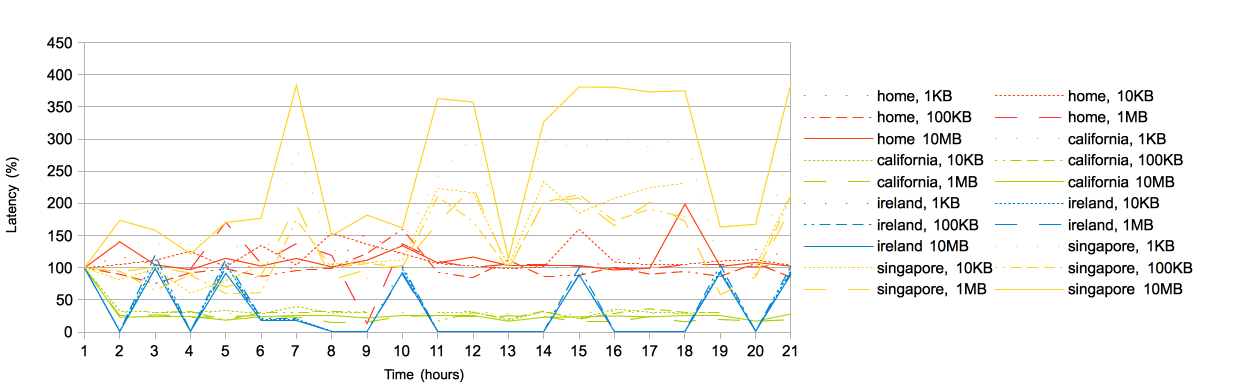
\includegraphics[width=\linewidth]{images/california_relative.png}
    \caption[]{Relative retrieval times using the California CloudFront distribution}
    \label{fig:california_relative}
\end{figure*}


\begin{figure*}[h]
    \centering
    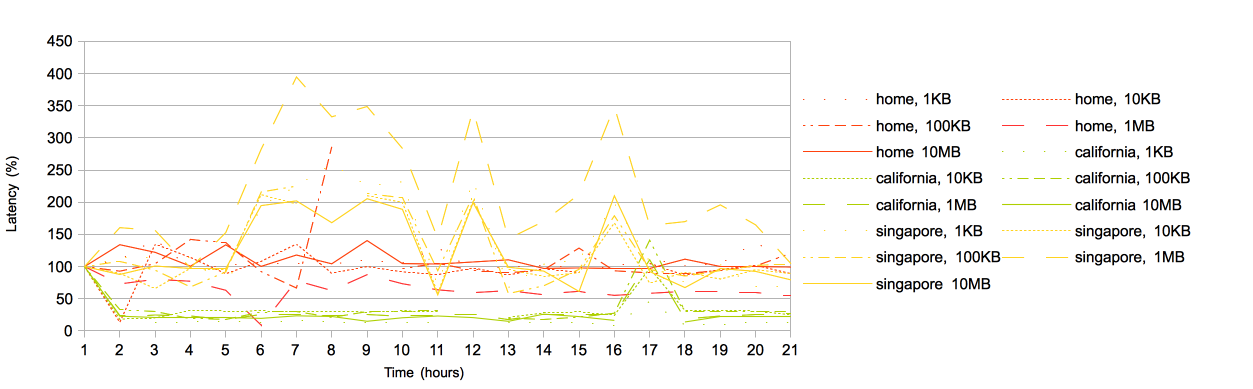
\includegraphics[width=7in]{images/ireland_relative.png}
    \caption[]{Relative retrieval times using the Ireland CloudFront distribution}
    \label{fig:ireland_relative}
\end{figure*}
\begin{figure*}[h]
    \centering
    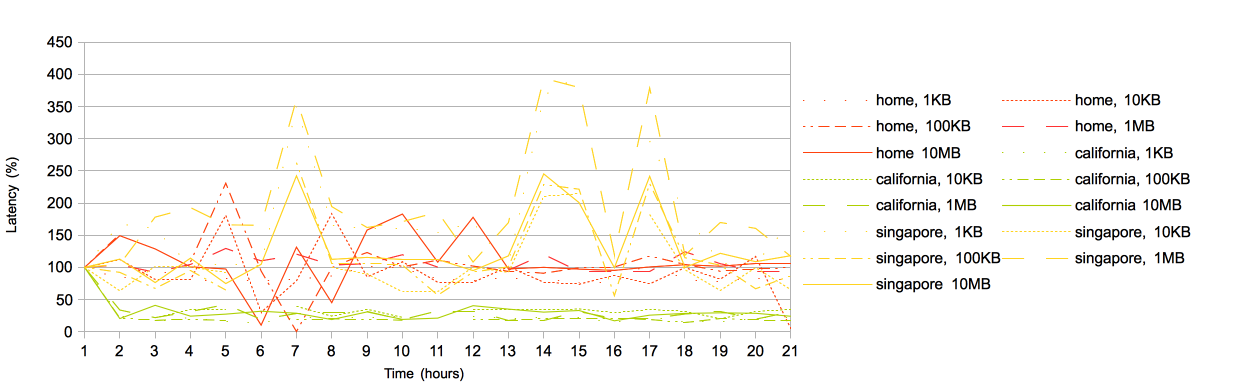
\includegraphics[width=7in]{images/tokyo_relative.png}
    \caption[]{Relative retrieval times using the Tokyo CloudFront distribution}
    \label{fig:tokyo_relative}
\end{figure*}
\begin{figure*}[h]
    \centering
    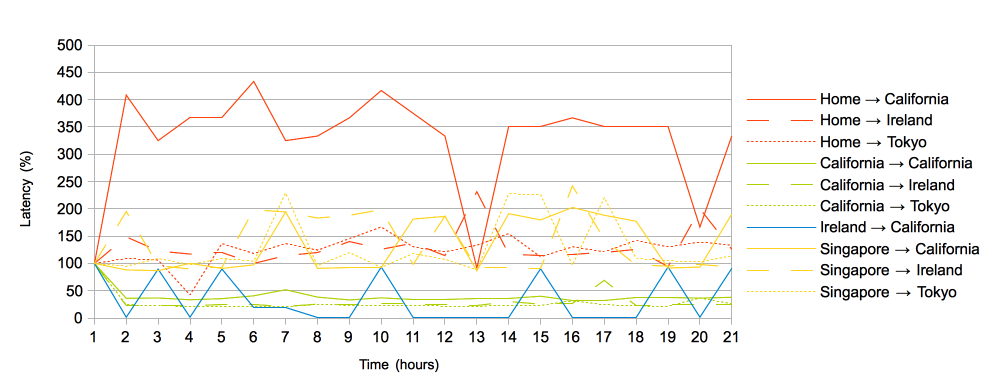
\includegraphics[width=7in]{images/pings_relative.png}
    \caption[]{Relative changes in network latencies}
    \label{fig:ping_relative}
\end{figure*}

\section{Analysis}
Network latencies should not change because of file propagation since the request goes always to the same host and responses directly regardless of cached files. So what then causes the changes in the network latencies? One reason is that the level of congestion between hosts simply varies. This is, however, not enough to explain the huge changes in case of Ireland, for example. How could the latency always increase to nearly exactly the same level? We were not able to answer to this question. Another open question is that why is the network latency from California EC2 to California cloudfront distribution constantly higher than to Ireland and Tokyo?




% An example of a floating figure using the graphicx package.
% Note that \label must occur AFTER (or within) \caption.
% For figures, \caption should occur after the \includegraphics.
% Note that IEEEtran v1.7 and later has special internal code that
% is designed to preserve the operation of \label within \caption
% even when the captionsoff option is in effect. However, because
% of issues like this, it may be the safest practice to put all your
% \label just after \caption rather than within \caption{}.
%
% Reminder: the "draftcls" or "draftclsnofoot", not "draft", class
% option should be used if it is desired that the figures are to be
% displayed while in draft mode.
%
%\begin{figure}[!t]
%\centering
%\includegraphics[width=2.5in]{myfigure}
% where an .eps filename suffix will be assumed under latex,
% and a .pdf suffix will be assumed for pdflatex; or what has been declared
% via \DeclareGraphicsExtensions.
%\caption{Simulation Results}
%\label{fig_sim}
%\end{figure}

% Note that IEEE typically puts floats only at the top, even when this
% results in a large percentage of a column being occupied by floats.


% An example of a double column floating figure using two subfigures.
% (The subfig.sty package must be loaded for this to work.)
% The subfigure \label commands are set within each subfloat command, the
% \label for the overall figure must come after \caption.
% \hfil must be used as a separator to get equal spacing.
% The subfigure.sty package works much the same way, except \subfigure is
% used instead of \subfloat.
%
%\begin{figure*}[!t]
%\centerline{\subfloat[Case I]\includegraphics[width=2.5in]{subfigcase1}%
%\label{fig_first_case}}
%\hfil
%\subfloat[Case II]{\includegraphics[width=2.5in]{subfigcase2}%
%\label{fig_second_case}}}
%\caption{Simulation results}
%\label{fig_sim}
%\end{figure*}
%
% Note that often IEEE papers with subfigures do not employ subfigure
% captions (using the optional argument to \subfloat), but instead will
% reference/describe all of them (a), (b), etc., within the main caption.


% An example of a floating table. Note that, for IEEE style tables, the
% \caption command should come BEFORE the table. Table text will default to
% \footnotesize as IEEE normally uses this smaller font for tables.
% The \label must come after \caption as always.
%
%\begin{table}[!t]
%% increase table row spacing, adjust to taste
%\renewcommand{\arraystretch}{1.3}
% if using array.sty, it might be a good idea to tweak the value of
% \extrarowheight as needed to properly center the text within the cells
%\caption{An Example of a Table}
%\label{table_example}
%\centering
%% Some packages, such as MDW tools, offer better commands for making tables
%% than the plain LaTeX2e tabular which is used here.
%\begin{tabular}{|c||c|}
%\hline
%One & Two\\
%\hline
%Three & Four\\
%\hline
%\end{tabular}
%\end{table}


% Note that IEEE does not put floats in the very first column - or typically
% anywhere on the first page for that matter. Also, in-text middle ("here")
% positioning is not used. Most IEEE journals/conferences use top floats
% exclusively. Note that, LaTeX2e, unlike IEEE journals/conferences, places
% footnotes above bottom floats. This can be corrected via the \fnbelowfloat
% command of the stfloats package.



\section{Conclusion}


% conference papers do not normally have an appendix


% trigger a \newpage just before the given reference
% number - used to balance the columns on the last page
% adjust value as needed - may need to be readjusted if
% the document is modified later
%\IEEEtriggeratref{8}
% The "triggered" command can be changed if desired:
%\IEEEtriggercmd{\enlargethispage{-5in}}

% references section

% can use a bibliography generated by BibTeX as a .bbl file
% BibTeX documentation can be easily obtained at:
% http://www.ctan.org/tex-archive/biblio/bibtex/contrib/doc/
% The IEEEtran BibTeX style support page is at:
% http://www.michaelshell.org/tex/ieeetran/bibtex/
%\bibliographystyle{IEEEtran}
% argument is your BibTeX string definitions and bibliography database(s)
%\bibliography{IEEEabrv,../bib/paper}
%
% <OR> manually copy in the resultant .bbl file
% set second argument of \begin to the number of references
% (used to reserve space for the reference number labels box)
% \begin{thebibliography}{1}

% \bibitem{IEEEhowto:kopka}
% H.~Kopka and P.~W. Daly, \emph{Blah blah blah \LaTeX}, 3rd~ed.\hskip 1em plus
%   0.5em minus 0.4em\relax Harlow, England: Addison-Wesley, 1999.

% \end{thebibliography}


\bibliographystyle{IEEEtran}
\bibliography{references}

% that's all folks
\end{document}
